%# -*- coding: utf-8-unix -*-

\chapter{基于深度学习的网络流量异常检测算法改进与实现}

\section{基于深度学习模型——DNN的改进}
DNN,即深层神经网络,它包含多个非线性隐藏层,这使得它们能够在输入和输出之间学习到非常复杂的关系。根据神经元的特点,可以分为MLP、CNNs、RNNs等。本文构建了深层神经网络的MLP结构,下面给出在模型训练中的一些相关技术的阐述。

\subsection{Backpropagation(反向传播)}

Backpropagation,即反向传播,是一种用于人工神经网络的方法,它用于计算网络中要使用的权重的计算所需梯度。它经常用于训练深度神经网络,即DNN。反向传播技术是一种称为自动分化技术的特例。在深度学习过程中,反向传播通常被梯度下降优化算法所使用,用于通过计算损失函数的梯度来调整神经元的权重。这种技术也被称之为误差反向传输技术,因为误差是通过网络层在输出端计算出来的。反向传播需要每个输入值都有一个已知的期望输出值,因此它被认为是一种监督学习方法,但它也被用于一些无监督的网络如自动编码器。反向传播也是delta规则对多层前馈网络的推广,它使通过使用链式规则迭代计算每个层的梯度成为了可能。它与Gauss-Newton算法密切相关,是神经反向传播的一部分。反向传播可以被用于任何基于梯度的优化器,比如L-BFGS。

优化算法重复两个阶段的循环,传播和权重更新。当输入向量输入到网络中时,它会逐层向前传播,直到到达输出层。然后使用损失函数将网络的输出与期望的输出进行比较,为输出层中的每个神经元计算误差值。然后将误差值从输出反向传播回网络,直到每个神经元都有一个相关的误差值,这个值反映了该神经元对原始输出所做的贡献。反向传播使用这些误差值来计算损失函数的梯度。在第二阶段,这个梯度被馈送到优化器,优化器又用它来更新权重,以试图使损失函数最小化。

梯度优化算法:
$N$是一个神经网络,$e$为该网络的连接,$m$为输入$n$为输出。下面,$x_1,x_2,...$将表示向量$R^m$,$y_1,y_2,...$将表示向量$R^n$,$w_0,w_1,w_2,...$将表示向量$R^e$。这些分别称为:输入、输出和权重。

该神经网络对应于一个函数$y = f_N(w,x)$,给定一个权重$w$,会将输入$x$映射为输出$y$。

该算法将输入一系列训练样本$(x_1,y_1),...,(x_n,y_n)$,并将根据初始权重$w_0$(初始权重通常为随机选择)产生一系列权重$w_0,w_1,...,w_n$。

这些权重将依次被计算:首先只使用$(x_i,y_i,w_{i-1})$计算$w_i$,以此类推,将$i = 1,...,n$全部计算完毕。算法将输出$w_p$,同时给出我们一个新的函数$x \mapsto f_N(w_p,x)$。每一步的计算过程都像这样,所以在此只描述$i = 1$的情况。通过可变权重$w$来完成从$(x_1,y_1,w_0)$计算$w_1$,并且从$w = w_0$开始,应用梯度下降寻找函数$w \mapsto E(f_N(w,x_1),y_1)$的局部最小值。

这就是通过使用梯度下降寻找$w_1$的最小权重的方法。

学习算法:
为了实现上述算法,函数$w \mapsto E(f_N(w,x),y)$的梯度需要有明确的公式:$E(y,{y}') = \left |y - {y}'  \right |^2$。
学习算法分为两个阶段:传播和权重更新。
\begin{enumerate}
    \item 传播:每次传播都涉及以下两个步骤
    \begin{enumerate}
        \item 通过网络前向传播生成输出值。
        \item 计算误差。
        \item 利用训练数据的预期值,通过网络传播进行激活,以生成所有输出和隐藏神经元的增量(预期值和实际输出值之间的差值)。
    \end{enumerate}
    \item 权重更新:对于每项权重,必须依照如下步骤进行更新。
    \begin{enumerate}
        \item 权重的输出增量和输入激活被相乘,以找到权重的梯度。
        \item 从权重中减去权重梯度的比例,以百分比的方式。
        这个比率(百分比)影响学习的速度和质量,叫做学习速率。比率越大,训练的越快,比率越小,训练的准确度越高。权重梯度的正负表示与误差成正比或者反比。重复一定次数,直到网络被充分训练,达到我们的期望。
    \end{enumerate}
\end{enumerate}

传统的反向传播算法存在着一些问题,反向传播的梯度下降不能保证找到误差函数的全局最小值,只能得到局部最小值,同时在误差函数的横向传播上也很困难。反向传播算法不需要对输入向量进行归一化处理,然而,归一化处理可以提升训练的效果。反向传播算法在深度学习提出之前只能用于浅层的机器学习,一但层数增多,深度加深,反向传播算法的训练量将变得非常大,训练时间将变得非常长,在训练过程中还容易造成训练过拟合。鉴于这种情况,Hinton教授提出里一些改善这种问题的方法,使深度学习成为了可能。这些方法包括:使用随机梯度下降算法、使用Mini-batch技术、使用Dropout技术等。

\subsection{Dropout}
具有大量参数的深度神经网络是一种非常强大的深度学习系统,然而,这种系统中存在着严重的过拟合问题。由于有大量参数的存在,导致这种大型的深度学习系统非常慢,在测试时通过组合多种大型神经网络的预测来解决过拟合问题也变得十分困难。Dropout是解决这个问题的一项技术,它的核心思想是在神经网络的训练过程中,随机丢弃一些神经单元(连带着它们的连接),这样就可以防止模型的过度拟合。在训练过程中,从一个指数级数量的更瘦的网络中丢弃样本。在测试时,只需要简单地使用一个单一的有更小的权重的未稀释的网络,就可以很容易地估计出所有这些变瘦的网络的预测平均值。这显著减少了过拟合现象,并且比其它的正则化方法有了重大改进。这一技术的诞生,使神经网络在图像识别、文档分类、语音识别和计算生物学等监督学习任务中的表现得到了很大的提升,在很多基准数据集上也取得了十分突出的效果。
Dropout指在神经网络中丢弃一些单元(包括隐藏单元和可见单元)。丢弃的这些单元(包括其传入和传出的连接)是暂时的,随机的。丢弃的方法是在神经网络训练过程中,Dropout随机将一些节点的权重置为0,暂时不参加网络的计算,但是这些节点的自身的权重仍然保留着。这样,每次Dropout过后,都相当于在原始网络的基础上得到了一个更瘦的网络。如下图:
\begin{figure}[H]
    \centering
    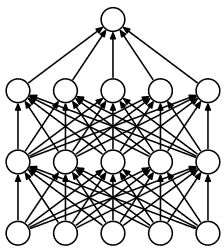
\includegraphics[width=0.5\textwidth]{dropout-before.png}
    \caption{原始网络}
    \label{fig:dropout-before}
\end{figure}
\begin{figure}[H]
    \centering
    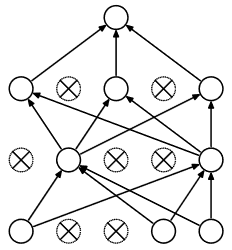
\includegraphics[width=0.5\textwidth]{dropout-after.png}
    \caption{Dropout后的网络}
    \label{fig:dropout-after}
\end{figure}

\subsection{Mini-batch}

在深度学习中,mini-batch也称分批处理,每一次epoch中所有的mini-batch的平均损失函数值就是它的错误率。相对于mini-btach的是full-batch,full-batch表示的是完整的数据集,每一次epoch中整个full-batch的损失函数值表示其错误率。

一般情况下,神经网络的权重更新:
\begin{equation}
    w \rightarrow {w}' = w - \eta \frac{\partial E}{\partial W}
\end{equation}

采用mini-batch的方法时,神经网络的权重更新方式则变为(假设mini-batch值为32):
\begin{equation}
    w \rightarrow {w}' = w - \eta \frac{1}{32} \frac{\partial E}{\partial W}
\end{equation}

即对每32个样本求其梯度的平均值,采用mini-batch的方法时,一个batch的所有数据放在了一个矩阵中,可以使梯度的计算速度大大加快,也就是说,整个深度学习网络的训练将会加快。在使用mini-batch的时候,batchsize的选取也没有一个固定的值,选取一个较大的batchsize,可以加快训练速度,但是这会造成权重的更新频率降低,降低了训练模型的收敛能力。另一方面,选取一个较小的batchsize,可以提高模型的收敛效果,但也会导致训练时间的延长。在实际应用中,往往需要我们根据模型的表现以及数据集的大小来确定batchsize的值。

\subsection{Batch Normalization}
在机器学习领域,往往在训练开始之前,需要对训练数据进行预处理,减均值,zscore,白化这三种方法可以逐级的提升随机初始化的权重对数据分割的有效性,同时可以降低过拟合的可能性。然而,在深度学习中,网络的深度是非常深的,如果对每一层的数据都进行这种处理,训练时间将会极大地延长。Google提出的Batch Normalization方法,给出了解决这一问题的方法。
该方法给出了如下改进:
\begin{enumerate}
    \item 单独对输入数据的每个维度进行规范化。
    \item 使用mini-batch中计算得到的均值与方差替代数据集整体的均值和方差。
\end{enumerate}

按照以往的理论来讲,对数据的预处理应当在每一层的激活函数之后进行,如在$ReLU=max(Wx+b,0)$之后,对数据进行归一化。然而,BN算法指出,这样做的话,在训练刚开始的情况下,分界面正在进行剧烈变化,此时计算出的参数不稳定,所以应当在$Wx+b$之后进行归一化。因为如果初始的$W$是从标准高斯分布中采样得到的,而$W$中元素的数量会远大于$x$,$Wx+b$每一维的均值本身就接近0、方差接近1,所以在$Wx+b$后使用Batch Normalization可以得到更稳定的结果。训练算法如下:
\begin{figure}[H]
    \centering
    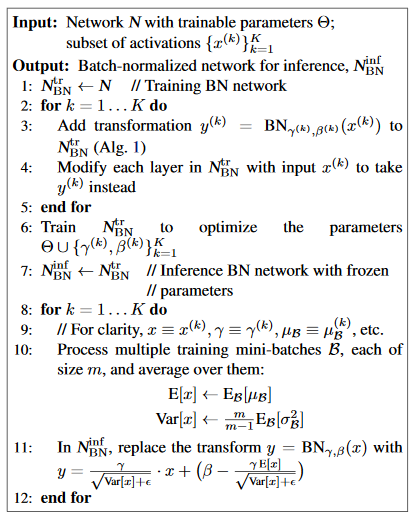
\includegraphics[width=0.5\textwidth]{BN.png}
    \caption{训练一个Batch Normalization网络}
    \label{fig:BN}
\end{figure}
在Normalization完成后,为了使数值的稳定性进一步加强,又加入了两个参数$\gamma$和$\beta$,使得:
\begin{equation}
    y^{(k)} = \gamma ^{(k)}\check{x}^{(k)} + \beta ^{(k)}
\end{equation}

这中算法带来了以下优势:
\begin{enumerate}
    \item 可以使用更高的学习率。
    \item 移除或使用较低的dropout。
    \item 降低L2权重衰减系数。
    \item 取消Local Response Normalization层。
    \item 减少图像扭曲的使用。
\end{enumerate}

\subsection{随机梯度下降算法}

随机梯度下降法(通常简称为SGD),也称为增量梯度下降法,SGD的主要思想是随机选取一个点做梯度下降,而不是遍历所有样本后进行参数迭代。因为梯度下降法的代价函数计算需要遍历所有样本,而且是每次迭代都要遍历,直至达到局部最优解,在样本量庞大时就显得收敛速度比较慢了,计算量非常庞大。随机梯度下降仅以当前样本点进行最小值求解,虽然通常无法达到真正局部最优解,但可以做到十分的接近最优解。

随机梯度下降算法的基本步骤是:
\begin{enumerate}
    \item 选择一个参数$w$和学习速率$\eta$的初始向量。
    \item 重复下列操作直到获取到近似最小值:
    \begin{enumerate}
        \item 在训练集中随机调整数据。
        \item $w := w - \eta \bigtriangledown Q_i(w)$,其中,$i = 1,2,...,n$
    \end{enumerate}
\end{enumerate}

随机梯度下降算法解决了收敛速度慢以及容易陷入局部最优解的问题。

\section{算法流程}

\section{实验数据集}

\subsection{数据集介绍}

KDD Cup 99数据集是使用1998年DARPA IDS评估计划捕获的网络流量制定的。1998年,美国国防部高级规划署(DARPA)在MIT林肯实验室进行了一项入侵检测评估项目。林肯实验室建立了一个模拟美国空军局域网的网络环境,以原始tcpdump格式的形式收集为期七周的用于训练的网络流量,然后是为期两周的用于测试的网络流量。这九周时间内手机的网络流量主要是网络连接和系统审计数据,包括正常流量和不同种类的攻击流量,仿真了各种用户类型、各种不同的网络流量和攻击手段,如DoS,Probing。测试数据包含许多在训练数据收集阶段未注入的攻击,使得入侵检测任务切合实际,据信,大多数新型攻击都可以从已知的攻击中获得。之后,训练和测试数据分别被处理成500万和200万个TCP/IP连接记录的数据集。KDD Cup数据集在NIDS评估中已被广泛用作多年的基准数据集。

一个网络连接定义为在某个时间内从开始到结束的TCP数据包序列,并且在这段时间内,数据在预定义的协议下(如TCP、UDP)从源IP地址到目的IP地址的传递。每个网络连接被标记为正常(Normal)或者异常(Attack),异常类型的连接被细分为4大类共39种攻击类型,其中22种攻击类型出现在了训练数据集中,其它的17种未知攻击类型被收纳在测试数据集中。详细的样本类别如下图:
\begin{figure}[H]
    \centering
    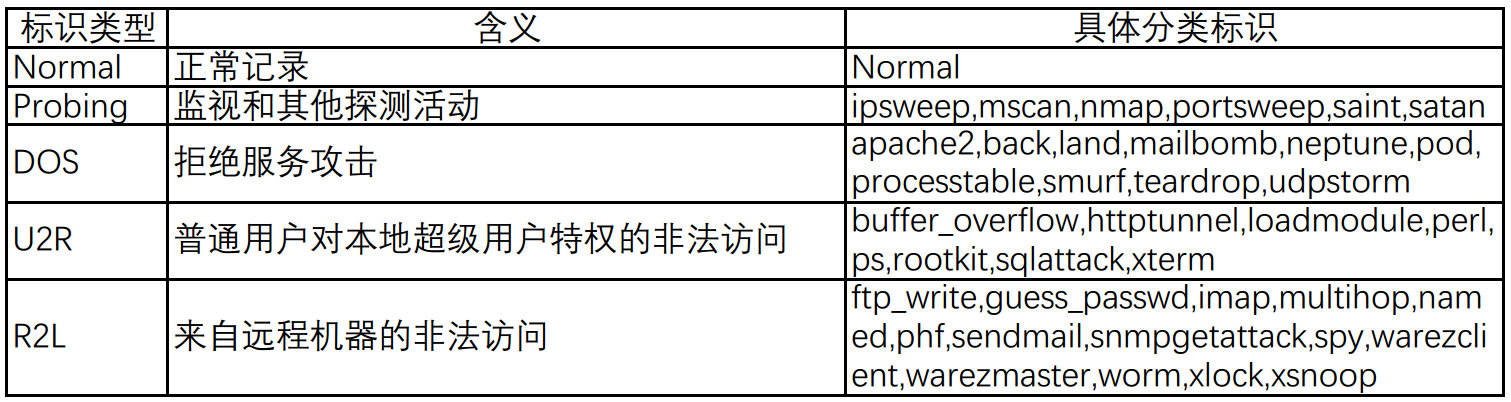
\includegraphics[width=0.99\textwidth]{kdd-classes.png}
    \caption{KDD Cup 99数据类别详情}
    \label{fig:kdd-classes}
\end{figure}

KDD Cup 99数据集中的每条连接都由41个特征组成,加上最后的标记数据,一共有42项的值:
\begin{figure}[H]
    \centering
    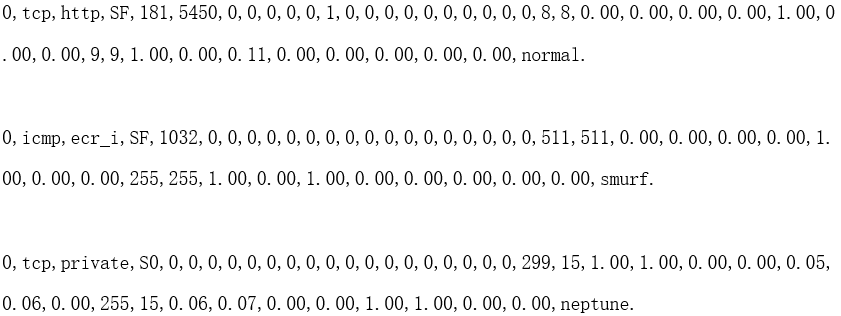
\includegraphics[width=0.99\textwidth]{kdd-data.png}
    \caption{KDD Cup 99数据类别详情}
    \label{fig:kdd-data}
\end{figure}

\subsection{数据预处理}

从上面的介绍中可以得知,深度学习在训练开始之前是需要对数据进行预处理的,KDD Cup 99数据集有41列特征以及一列标签,下面将阐述对数据进行的预处理操作。

数据预处理分两个阶段进行:
\begin{enumerate}
    \item 符号特征的数字化:

    数据集中有三列特征是符号类型的,符号特征的数字化也就是要将这些符号类型的特征转换成二进制的数字特征,方便机器理解与处理。将3种协议类型TCP,UDP,ICMP转换为二进制特征矢量分别是:TCP{1,0,0},UDP{0,1,0},ICMP{0,0,1}。按照这种方法,接下来将服务类型特征以及状态标志特征分别进行这种转换,其中,服务类型特征由1维转换为70维,状态标志特征由1维转换为11维。最终,数据集中的41维特征转换为了122维特征。

    数据集的最后一列是标签列,这一类也是符号特征,我将这列符号特征以两种不同的方式进行了数字化,首先,将标签数据分为了五种:Normal,PROBE,DOS,U2R,R2L分别对应0,1,2,3,4转换为了数字。又将标签数据分为了两种:正常(Normal)和异常(Attack),分别对应0和1,按这种方式转换为了数字。这么转换的原因是因为在实验中,我将分别测试模型对于2分类和5分类的准确率。

    \item 数字特征的归一化:

    本文对转换为数字特征的全部122维数据按照下面的公式进行了归一化处理:
    \begin{equation}
        output = \frac{y - X_{min}}{X_{max} - X_{min}}
    \end{equation}
    其中,$output$为归一化后的输出结果,$y$为将要被归一化的数字,$X_{min}$为$y$所在的这一维度中的最小值,$X_{max}$为$y$所在的这一维度中的最大值。本文最终选用了KDD Cup 99数据集中的“KDD 10\%”和“corrected”这两个数据集作为训练和测试数据集。这两个数据集的统计信息如下:
    % Table generated by Excel2LaTeX from sheet 'Sheet2'
    \begin{table}[htbp]
        \centering
        \caption{KDD Cup 99数据集统计信息}
        \begin{tabular}{c|c|c|c|c|c|c}
            \toprule
            KDD Cup 99 & All types & NORMAL & PROBE & DOS    & U2R & R2L   \\
            \midrule
            KDD 10\%   & 494021    & 97278  & 4107  & 391458 & 52  & 1126  \\
            \midrule
            corrected  & 311029    & 60593  & 4166  & 229853 & 228 & 16189 \\
            \bottomrule
        \end{tabular}%
        \label{tab:kdd-dataset-info}%
    \end{table}%
\end{enumerate}

\section{本章小结}

本章首先讲解了深度学习模型——DNN所依赖的关键技术,其中包括BP、Dropout、Mini-batch、BN和SGD,正是因为这些优秀的算法,才能使得深度学习的训练称为可能。紧接着使用伪代码的形势描述了本文基于深度学习的网络流量异常检测算法的算法流程,最后对实验所选用的数据集——KDD Cup 99入侵检测数据集进行了详细的介绍,同时也给出了对数据集的数据进行预处理和归一化的方法。
